\documentclass[a4paper,12pt]{report}

\usepackage[serbian, ngerman, english]{babel}
\usepackage[a4paper, inner=3cm, outer=3cm, top=2cm, bottom=2cm]{geometry}
\usepackage{blindtext}
\usepackage{microtype}
\usepackage{graphicx}
\usepackage{wrapfig}
\usepackage{enumitem}
\usepackage{fancyhdr}
\usepackage{amsmath}
\usepackage{index}
\usepackage[autostyle]{csquotes}
\usepackage{amssymb}
\DeclareMathOperator*{\argmax}{argmax}
\usepackage{listings}
%\usepackage{booktabs}

\makeindex
%after this beguins the document

\begin{document}
\selectlanguage{serbian} 
%\renewcommand{\contentsname}{Sadržaj}
%\renewcommand{\chaptername}{Poglavlje}

\title{\Large{\textbf{Logistička i softmaks regresija (opis metoda, implementacija, primena nad podacima, komparativna analiza) i njihova primena kao aktivacione funkcije u neuronskim mrežama }}}
\author{Student: Danilo Veljović, broj indeksa: 1120}
\date{Novembar 6, 2020}
\maketitle
\let\cleardoublepage\clearpage
\tableofcontents

\pagenumbering{arabic}

\setcounter{page}{1}

\chapter{Uvod}
\ Termini poput veštačke inteligencije i mašinskog učenja su sve popularniji u savremenoj kulturi. Preko medija sve češće čujemo nagoveštaje vodećih naučnika iz ove oblasti da će sistemi koji koriste veštačku inteligenciju zameniti ljude na mnogim radnim mestima. Priča se da će prvo nestati najrepetitivniji poslovi poput vozača kamiona, radnika u skladištima, prodavaca i dr. Treba postaviti suštinsko pitanje zašto je to tako. Zašto će prvo rutinski poslovi nestati prvi? Odgovor na to pitanje daje prave smernice kada neko pokušava da shvati šta je to mašinsko učenje. \\ 

Mašinsko učenje vuče korene iz statistike. Slobodno rečeno, mašinsko učenje se može shvatiti kao primena statističkih metoda nad velikom količinom podataka, da bi se izvukle nekakve pravilnosti iz podataka. Te pravilnosti uočava model i opisuje ih različitim statističkim terminima. Model se može shvatiti kao parametrizovana funkcija koja može da \enquote{uči} iz podataka. Podaci se u mašinskom učenju dele na trening i test skupove. Trening skupovi imaju određene vrednosti za atribute i imaju izlaznu labelu klase kojoj pripadaju ili neke kontinualne vrednosti koju uzimaju. Model uzima jedan po jedan podatak iz trening skupa, ili čitavu grupu, i proba da napravi predikciju koje bi izlazne vrednosti mogle da odgovaraju tim ulazima. Kada vidi koliko njegova procena odudara od vrednosti labele za taj podatak, on se ispravi svoje parametre. Ovaj proces se naziva treniranje modela. Kada model optimizuje svoje parametre, i kada se odradi evaluacija modela, prelazi se na testiranje. Kada se model testira njemu se daju instance podataka koje nikad nije video. Za te instance on sada predviđa izlazne labele. \\

Posle ovog kratkog objašnjenja procesa mašinskog učenja, lako se može naslutiti odgovor na prethodno postavljeno pitanje o poslovima koje će prvo 
\enquote{progutati} inteligentni sistemi. Uzmimo primer radnika koji radi u skladištu i pomera kutije od mesta A do mesta B. Robot može da posmatra radnika koji nosi kutije i da zaključi da radnik na mestu A podigne kutiju, nosi je do mesta B i tu je spušta. To je njegov \enquote{trening skup} podataka. Kod ovakvog tipa inteligentih sistema najčešće se koriste konvolucione neuronske mreže za računarski vid, pomoću kojih sistem prima podatke o tome šta se dešava oko njega. Princip ostaje isti, sistem preko kamera, prima ulazne podatke, i ovo služi kao trening skup podataka. Trenira određen model, i kada se završi taj proces on može da izvede zadatak prenosa kutija. Ako se od sistema zahteva da radi nešto novo, slično prethodnom, on će probati to da uradi na jedan način, i u zavisnosti od ishoda \enquote{učiće} o tome gde je pogrešio, odnosno optimizovaće model. \\

%sad malo o konkretnim tehnikama, logističkoj, softmaks regresiji i pregled rada nadalje
Tehnike mašinskog učenja su srž inteligentnih sistema. Neki od važnijih modela mašinskog učenja su: 
\begin{itemize}
	\item \textit{Klasifikacija} predviđa klasu koja odgovara podatku
	\item \textit{Regresija} predviđa kontinualnu vrednost koja odgovara podatku
	\item \textit{Klasterizacija} je tehnika nenadgledanog učenja. Za razliku od tehnika nadgledanog učenja, o kojima je do sad bilo reči, kod nenadgledanog učenja nemamo informaciju o tome koji podatak ima kakvu klasu/vrednost. Zadatak klasterizacije je da one podatke koji su \enquote{slični} (mera sličnost se definiše kao parametar tehnike) grupiše zajedno.
	\item \textit{Neuronske mreže} su tehnika koja je donela revoluciju u svet mašinskog učenja i omogućila stvari poput računarskog vida i procesuiranja prirodnih jezika. Ideja za ovu tehniku dobijena je iz ideje ljudskog mozga. Cela neuronska mreža se sastoji iz veštačkih neurona, koji su međusobno povezani. Na slici 1.1 dat je prikaz jedne neuronske mreže. Neuronska mreža se sastoji iz tri sloja, \textit{ulaznog} sloja, mnoštvo \textit{skrivenih} slojeva i \textit{izlaznog sloja}. Ideja kod funkcionisanja neuronske mreže je da početni slojevi prepoznaju jako male delove sistema, npr kod računarskog vida prepoznaju ivice, kod procesuiranja prirodnih jezika prepoznaju pojedina slova. Skriveni slojevi prepoznaju složenije pojave, npr geometrijske figure ili tela, ili reči i rečenice. Na kraju izlazni neuroni se aktiviraju ako je prepoznato nešto. Primera radi, mreža može da se trenira da prepoznaje slike mačaka ili da prepoznaje da li je neka rečenica nosi pozitivna ili negativna osećanja. Ako mreža prepozna sliku mačke, ili ako je određena rečenica ima pozitivna osećanja, izlazni neuron se aktivira. 
\end{itemize}

\begin{figure}[ht]
	\centering
	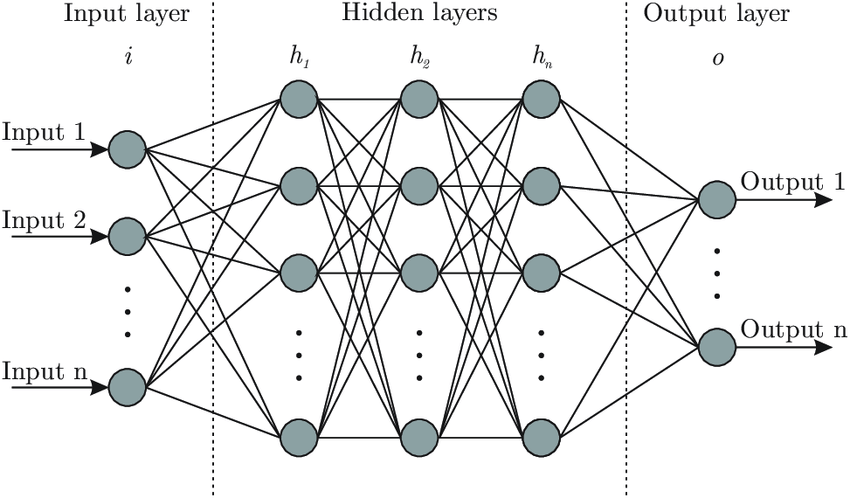
\includegraphics[width=8cm]{neuronske_mreze.png}
	\caption{Arhitektura neuronske mreže}\label{fig:prettypic}
\end{figure}

Jedna od tehnika koja se koristi za klasifikaciju se naziva \textit{logistička regresija}. Iako u nazivu sadrži reč \textit{regresija} ova tehnika se ne koristi za predviđanje kontinualne vrednosti, već za predviđanje da li neki podatak pripada nekoj klasi ili ne. U nastavku rada biće reči o matematičkim osnovama logističke regresije, o funkciji koja je vrlo slična logističkoj regresiji i vrlo često se koristi u sličnim situacijama - \textit{softmaks regresiji}. Implementiraćemo logističku i softmaks regresiju u programskom jeziku Python, primeniti je nad skupom podataka i evaluirati njihove performanse i napraviti komparativnu analizu obe tehnike. Na kraju rada biće dat prikaz primene logističke i softmaks regresije kao 
aktivacione funkcije (\enquote {\textit{threshold functions}}) kod neuronskih mreža.
\chapter{Teorijske osnove}

\section{Kratak pregled potrebnih pojmova iz verovatnoće i statistike}
Kako bi se pravilno razumela logistička regresija potrebno je pre toga dobro poznavati njene matematičke osnove. U nastavku je data kratka rekapitulacija potrebnih pojmova iz verovatnoće i statistike koji su potrebni za njeno razumevanje. Da bi se lakše svi pojmovi dati u nastavku, razmatrani su samo u okvirima diskretnih slučajnih promenljivih.\\

\subsection{Verovatnoća} 
Verovatnoća predstavlja odnos između broja ishoda u kome je neki događaj ispunjen i broja svih mogućih ishoda. 
\begin{equation} \label{eq:1}
	P = \frac{\textit{broj pozitivnih ishoda događaja}}{\textit{broj svih mogućih ishoda}} 
	%\caption{}
 \end{equation}
 
 \textit {Primer 1.} \
Primer jednog događaja može biti bacanje novčića. Pozitivan ishod je kada se padne glava. Broj svih mogućih ishoda u jednom bacanju je 2 (može se pasti ili pismo ili glava). Kada zamenimo ove vrednosti u prethodnu jednačinu dobijamo: 
\begin{equation} \label{eq:2}
	P = \frac{1}{2} = 0.5
	%\caption{}
 \end{equation}
Iz jednačine se vidi da je verovatnoća da u jednom bacanju novčića dobijemo glavu 0.5, odnosno 50 \%.

\subsection{Šansa}

Šansa predstavlja odnos između verovatnoće da se događaj desio i verovatnoće da se događaj nije desio.
\begin{equation} \label{eq:3}
	\textit{šansa} = \frac{\textit{P(događaj se desio)}}{\textit{P(događaj se nije desio)}} = \frac{\textit{p}}{\textit{1-p}}
	%\caption{}
 \end{equation}

Ako se vratimo na primer 1 bacanja novčića, vidimo da je šansa da se događaj desi, odnosno da se padne glava jednak: 
\begin{equation} \label{eq:4}
	\textit{šansa(glava)} = \frac{0.5}{0.5} = 1, tj. \textit{1:1}
	%\caption{}
 \end{equation}
 
 Zaključujemo da je šansa da se padne glava ista kao i šansa da se ne padne glava, tj 1 prema 1. 
 
 Odnos šansi se definiše kao:
 \begin{equation} \label{eq:4}
	\textit{odnos šansi} = \frac{\textit{šansa\textsubscript{1}}}{\textit{šansa\textsubscript{1}}} 
	%\caption{}
 \end{equation}
 
 \textit {Primer 2.} \ Uzmimo dva novčića, jedan koji je fer i drugi za koji se zna da je verovatnoća da se padne glava 0.7. Naći odnos šansi ova dva novčića za događaj kada se padne glava.\\
 Za fer novčić važi: 
 \begin{equation}
	P(glava) = \frac{1}{2} = 0.5 \\
	%\caption{}
 \end{equation}
 \begin{equation}
	\textit{šansa(glava)\textsubscript{fer}} = \frac{0.5}{0.5} = 1, tj. \textit{1:1}
	%\caption{}
 \end{equation}
 
 Za \enquote{nefer} novčić važi: 
  \begin{equation}
	P(glava) = 0.7
	%\caption{}
 \end{equation}
 \begin{equation}
	\textit{šansa(glava)\textsubscript{nefer}} = \frac{0.7}{0.3} = 2.333
	%\caption{}
 \end{equation}
 
 Odnos šansi definišemo kao: 
  \begin{equation}
	 \textit{odnos šansi} = \frac{\textit{šansa(glava)\textsubscript{nefer}}}{\textit{šansa(glava)\textsubscript{fer}}} = \frac{2.333}{1} = 2.333
 \end{equation}
 Vidi se da su šanse da se padne glava na \enquote(nefer) novčiću veća nego da se dobije glava na \enquote(fer) novčiću 2.333 puta. 
\subsection{Bernulijeva raspodela}

Bernulijevu raspodelu je najlakše razumeti kroz Bernulijev eksperiment. Bernulijev eksperiment je eksperiment koji se dešava jednom i koji kao rezultat može da ima uspeh (obično obeležen 1) ili neuspeh (obično obeležen 0) tj ima samo dve moguće posledice. Najbolji primer za to je bacanje novčića. Dve moguće posledice su da se padne ili pismo ili glava. Uzmimo da se uspešnim događajem smatra da se pala glava pri bacanju. Odavde sledi da ako se padne pismo, to smatramo neuspehom. Izvedemo eksperiment jednom i ako se padne glava smatramo da se desio uspešan događaj, ako se padne glava smatramo da se desio neuspešan događaj. \\

Definišemo slučajnu promenljivu $X$ = broj uspeha pri bacanju novčića i $X \sim Bernoulli(p)$. Moguće vrednosti koje slučajna promenljiva može da ima (obeležavamo ih sa x) su 0 ili 1. Nula se dobija ako se pri jednom bacanju nije desio uspešan događaj, odnosno 1 ako se desio uspešan događaj.  Obeležavamo to sa x = 0, 1. \\
Verovatnoća da se desio uspešan događaj je ujedno i jedini parametar distribucije, i obeležava se sa $p$.
  \begin{equation}
	 P(X = 1) = p 
 \end{equation}
Jedan parametar se prosleđuje jer imamo samo jedan eksperiment. Odavde se može primetiti da je Bernulijeva raspodela specijalan slučaj Binomne raspodele za $n = 1$.\\
Verovatnoća da se desio neuspešan događaj je:
\begin{equation}
	 P(X = 0) = 1-p = q 
 \end{equation}

Za primer fer bacanja novčića, verovatnoća uspeha je:
  \begin{equation}
	 P(X = 1) = 0.5 
 \end{equation}
Verovatnoća neuspeha je data u jednačini
  \begin{equation}
	 P(X = 0) = 0.5 
 \end{equation}
 
Očekivana vrednost (srednja vrednost) se za diskretne slučajne promenljive koje imaju Bernulijevu raspodelu dobija kao:  
   \begin{equation}
	 \mu = E[X] = \sum_{x\textsubscript{i} \in \mathcal{X}}^{\mathcal{X}} x\textsubscript{i} p(X = x\textsubscript{i}) = 1 * p + 0 * q = p
 \end{equation}

gde je $X$ slučajna promenljiva, $x$ moguće vrednosti slučajne promenljive i $\mathcal{X}$ je skup vrednosti koje slučajna promenljiva može da ima.\\

Varijansa (mera koja pokazuje meru odstupanja od srednje vrednosti) se dobija kao:
\begin{equation}
\begin{split}
Var[X] = \sigma^2 & =  \\
& = Cov[X, X] = \\
& = E[(X - \mu)(X - \mu)] = E[(X - \mu)^2] = \\ 
& = \sum_{x\textsubscript{i} \in \mathcal{X}}^{\mathcal{X}} (x\textsubscript{i} - \mu)^2 p(X = x\textsubscript{i}) = \\
& = (0 - p)^2 * q + (1 - p)^2 * p = p^2*q +  q^2*p = pq (p + q) = pq
 \end{split}
 \end{equation}
 
Standardna devijacija predstavlja koren iz varijanse:
\begin{equation}
\sigma = \sqrt{(Var[X])} = \sqrt{pq}
\end{equation}

\section{Logistička regresija}

Logistička regresija je tehnika koja se koristi za klasifikaciju. Najčešće primenu nalazi u binarnoj klasifikaciji. Pomoću nje se određuje da li neki podatak pripada nekoj klasi ili ne. Da bi se neki skup podataka mogao modelirati logističkom regresijom, on mora imati Bernulijevu raspodelu. U skladu s tim se očekuje da se na izlazu mogu pojaviti samo dve vrednosti. Nula na izlazu znači da podatak ne pripada klasi, dok jedinica znači da podatak pripada klasi. 

\subsection{Procena verovatnoće}

\ Slično linearnoj regresiji, logistička regresija procenjuje nepoznatu verovatnoću linearne kombinacije elemenata ulaznog vektora. Nepoznatu verovatnoću procenjuje logističkom funkcijom. Nakon procene verovatnoće određene linearne kombinacije elemenata ulaznog vektora, mapira tu verovatnoću na 0 ili 1. Ako je procenjena verovatnoće \textit{p} veća od 0.5 daje izlaz 1, odnosno 0, ako je verovatnoća manja od 0.5. Procenjena verovatnoća \textit{p} se često obelažava sa \textit{\^{p}}. \\

\ Skup ulaznih podataka kod logističke regresije, bar u slučaju mašinskog učenja, predstavljen je kao matrica \textbf{$\theta^T$x}, gde je \textbf{x} = {x\textsubscript{1}, x\textsubscript{2}, ..., x\textsubscript{n}} a $\theta$ = {$\theta$\textsubscript{1}, $\theta$\textsubscript{2}, ..., $\theta$\textsubscript{n}}, odnosno \textbf{x} je vektor atributa podataka na ulazu, a $\theta$ su odgovarajuće težine svakog od atributa. \\

Potrebno je naći vezu između nezavisnih promenljivih na ulazu i izlaza tako da, kao kod Bernulijeve raspodele, izlaz bude ili 0 ili 1. Ta veza se predstavlja \textit{logit} funkcijom. Logit funkcija mapira linearnu kombinaciju nezavisno promenljivih na ulazu na izlaz . Logit funkcija predstavlja prirodni logaritam šanse. Logit funkcija je podobna jer ima samo jedan ulazni parametar koji ce kasnije biti verovatnoća p \\
\begin{equation}
\textit{logit(p)} = ln \left( \frac{\textit{p}}{\textit{1-p}} \right)
\end{equation}

Logit funkcija je data na slici 2.1. Domen funkcije je interval $ (0, +1) $, i definisana je svuda sem u 0 i 1. Kodomen funkcije je interval 
$ (-\infty, +\infty) $. Pošto je potrebno da nama argumenti mogu da uzmu bilo koju realnu vrednost, a da izlaz bude u intervalu između 0 i 1, potražićemo inverznu funkciju ovoj. Ta funkcija se naziva \textit{logistička} funkcija. Izvođenje je dato u jednačini 2.12. Finalni oblik logističke funkcije dat je u jednačini 2.13.

\begin{equation}
\begin{split}
ln \left( \frac{\textit{p}}{\textit{1-p}} \right) & = \alpha, \alpha \in \rm I\!R\\  
	\frac{p}{1-p} = e^\alpha\\
	p = e^\alpha(1-p)\\
	p + pe^\alpha - e^\alpha  = 0\\
	p(1+e^\alpha) - e^\alpha  = 0\\
	p  = \frac{e^\alpha}{1+e^\alpha}
\end{split}
\end{equation}

\begin{equation}\label{eq:hypothesis}
 logit^{-1}(\alpha) = h\textsubscript{$\theta$}(\alpha) = \sigma(\alpha) = \frac{e^\alpha}{1+e^\alpha} =\frac{1}{1+e^{- \alpha}}
\end{equation}
\begin{figure}
    \centering
    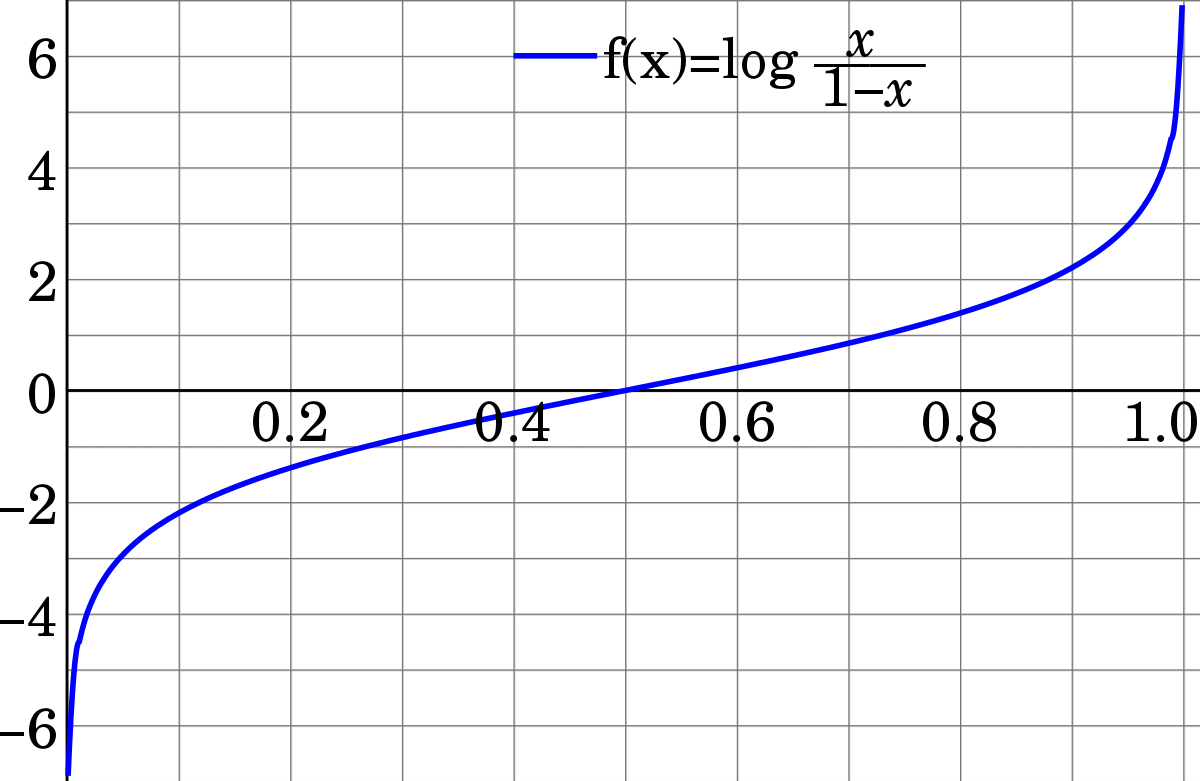
\includegraphics[width=0.5\textwidth]{logit.png}
    \caption{Logit funkcija}\label{fig:prettypic}
\end{figure}
\begin{figure}
    \centering
    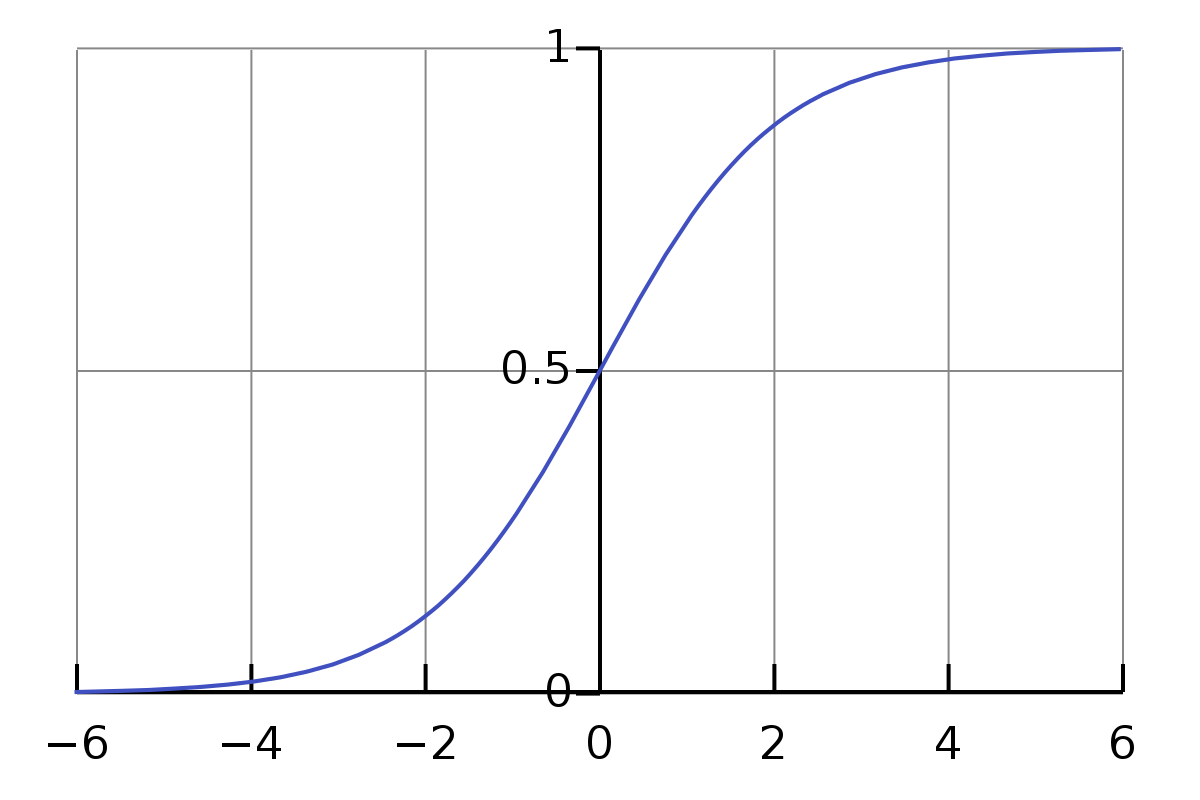
\includegraphics[width=0.5\textwidth]{logistic.png}
    \caption{Logistička funkcija}\label{fig:prettypic}
\end{figure}

Grafik logističke funkcije dat je na slici 2.2. Vidimo da je sada domen funkcije $ (-\infty, +\infty) $, a kodomen $ (0, +1) $. Ovakva funkcija se naziva \textit{sigmoidnom} funkcijom (takođe postoji naziv i \enquote{S}-kriva) i ona daje broj uvek između 0 i 1. \\
Kada logistička regresija nađe verovatnoću \textit{\^{p}} kao funkciju ulaznih parametara , ona na osnovu te verovatnoće može da da predikciju da li taj podatak pripada pozitivnoj klasi. 

\begin{equation}
  \textit{\^{y}} =
  \begin{cases}
    1, & \textit{\^{p}} > 0.5 \\
    0, & \textit{\^{p}} < 0.5
  \end{cases}
\end{equation}

\subsection{Treniranje modela i funkcija gubitka}

Cilj treniranja modela je da se podese parametri vektora  $\theta$ tako da model daje visoku verovatnoću za pozitivne instance (y = 1) i nisku verovatnoću za negativne instance (y = 0).  Funkcija gubitka se koristi kada se optimizuju parametri modela. Funkcija gubitka mapira neku realnu vrednost, najčešće je to nekakva razlika predviđene vrednosti i stvarne vrednosti labele neke instance, u realan broj. Taj realan broj predstavlja cenu. Cilj optimizacije modela je da minimizira funkciju gubitka. Početni izgled funkcije gubitka za logističku regresiju je dat u jednačini . 

\begin{equation} \label{eq:f-ja kostanja}
  \textit{c($\theta$)} =
  \begin{cases}
    -ln($\^{p}$), &  y = 1 \\
    -ln(1 - $\^{p}$), & y = 0
  \end{cases}
\end{equation}

\begin{figure}
    \centering
    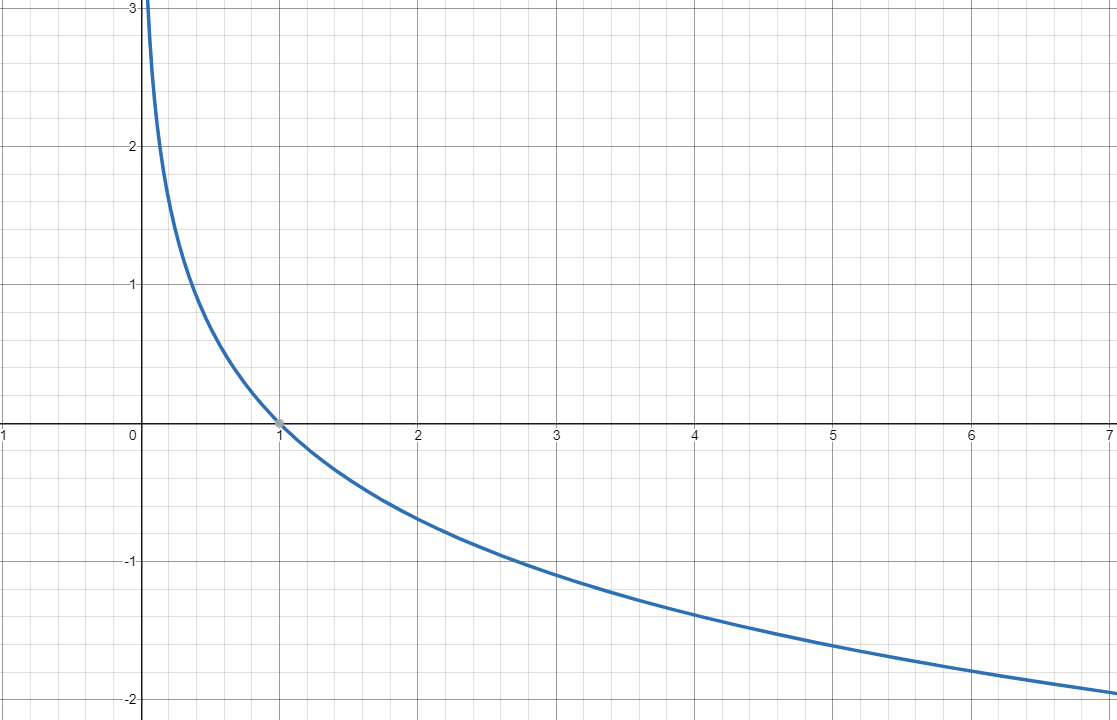
\includegraphics[width=0.5\textwidth]{neglog.png}
    \caption{Grafik funkcije -ln(x)}\label{fig:neglog}
\end{figure}

Na slici \ref{fig:neglog} je dat grafik funkcije $-ln(x)$. Kada $x \to 0$ , tada $ -ln(x) \to \infty $. Zbog toga će cena biti velika ako model proceni verovatnoću koja teži nuli za pozitivne instance. Takođe biće jako velika ako model proceni verovatnoću blizu jedinice za negativne instance. Ako je x u okolini jedinice, tada će -ln(x)  imati vrednost oko nule. Odnosno ako cena će biti 0 ako je procenjena verovatnoća blizu 0 za negativne instance, ili blizu 1 za pozitivne instance. Funkcija \ref{eq:f-ja kostanja} se može takođe napisati kao:
\begin{equation} \label{eq:logloss}
	 \textit{c($\theta$)} = [\ y ln(\hat{p}) + (1 - y)ln(1 - \hat{p}) ]\
\end{equation}
Odnosno za sve elemente ulazne matrice dobijamo konačni oblik, dat u jednačini \ref{eq:loglossfinal}. 
\begin{equation} \label{eq:loglossfinal}
	 J(\theta) = -  \frac{1}{m} \sum_{i=1}^{m} [\ y^i ln(\hat{p}^i) + (1 - y^i)ln(1 - \hat{p}^i) ]\
\end{equation}

Konstanta $\frac{1}{m}$ se koristi da bi se našla prosečna vrednost svih grešaka. Jednačina zatvorenog oblika koja optimalne izračunava vrednosti $\theta$ vektora nije poznata. Međutim ova funkcija jeste konveksna, tako da se optimizacionim algoritmom opadajućeg gradijenta može naći globalni minimum funkcije. Za globalni minimum funkcije gubitaka svi parametri vektora $\theta$ imaju optimalne vrednosti, odnosno najmanja je razlika između pravih labela i procenjenih labela. Kada se stigne do globalnog minimuma nije više moguće smanjivati razliku između procenjene i realne vrednosti. \\

U nastavku biće dat postupak dobijanja gradijenta funkcije \ref{eq:loglossfinal}. Biće dat postupak dobijanja parcijalnog izvoda po promenljivoj $\theta \textsubscript{j}$. Gradijent funkcije je specijalan slučaj Jakobijeve matrice, kada je funkcija skalarna. U opštem slučaju gradijent skalarne diferencijabilne funkcije više promenljih je vektorsko polje $ \nabla $ \textit{f} čija vrednost u tački \textit{p} je vektor čije komponente su parcijalni izvodi \textit{f} u \textit{p}. Odnosno za \textit{f}: $ \rm I\!R  ^ n \to \rm I\!R $, njen gradijent je definisan kao: $ \nabla $ \textit{f}: $ \rm I\!R  ^ n \to \rm I\!R ^ n $   je definisan u tački \textit{p} = (x\textsubscript{1}, x\textsubscript{2}, ..., x\textsubscript{n}) u n-to dimenzionalnom prostoru kao vektor:

\begin{equation}
\begin{split}
\nabla \textit{f(p)} = 
\begin{pmatrix} \frac{\partial f}{\partial x \textsubscript{1}} \\\\ \frac{\partial f}{\partial x\textsubscript{2}} \\.\\ .\\.\\ \frac{\partial f}{\partial x\textsubscript{n}} \end{pmatrix}
\end{split}
\end{equation}

Gradijent vektor se može protumačiti kao \enquote{pravac i stopa najbržeg rasta} funkcije. Ako je gradijent funkcije u tački \textit{p} nenulti, pravac gradijenta je pravac u kome funkcija najbrže raste od tačke \textit{p}. Intenzitet gradijenta je stopa rasta u tom pravcu. Gradijent je nulti vektor u tački samo ako je to stacionarna tačka, tj. ako je to tačka ekstremuma. Kasnije će biti potrebno da iterativnim metodama smanjujemo vrednost funkcije i za ovo će nam biti potreban negativan gradijent funkcije, umesto pozitivnog.\\

\textbf{Izvod logističke funkcije}\\

U nastavku je dat izvod logističke funkcije $\sigma(x)  = \frac{1}{1+e^{-x}}$.

\begin{equation}
\begin{split}
	\frac{\partial (\sigma(x))}{\partial x} & = \frac{0 * (1 + e^{-x}) - (1)*(e^{-x}*(-1))}{({1+e^{-x}})^2} \\
 		& = \frac{ e^{-x}}{({1+e^{-x}})^2} = \frac{1-1 + e^{-x}}{({1+e^{-x}})^2}= \frac{ 1 + e^{-x}}{({1+e^{-x}})^2} - \frac{1}{({1+e^{-x}})^2} \\
 		& = \frac{1}{1+e^{-x}} * \left( 1 - \frac{1}{1+e^{-x}}\right) = \sigma(x)(1-\sigma(x))
\end{split}
\end{equation}

\textbf{Izvod funkcije gubitaka}\\

U nastavku je dat izvod funkcije gubitaka \ref{eq:loglossfinal}.\\

\textbf{Korak 1: Nalaženje diferencijala složene funkcije:}

\begin{equation}
\begin{split}
	\frac{\partial (J(\theta))}{\partial \theta\textsubscript{j}} & = -  \frac{1}{m} \left( \sum_{i=1}^{m} \left[\ y^i * \frac{1}{h\textsubscript {$\theta$} (x^i)}  * \frac{\partial (h\textsubscript {$\theta$}(x^i)}{\partial \theta\textsubscript{j}}\right] + \sum_{i=1}^{m} \left[\ (1 - y^i) * \frac{1}{1 - h\textsubscript {$\theta$} (x^i)}    * \frac{\partial (1 -h\textsubscript {$\theta$}(x^i)}{\partial \theta\textsubscript{j}}\right]\ \right) \\
 		& = - \frac{1}{m} \left( \sum_{i=1}^{m} \left[\ y^i * \frac{1}{h\textsubscript {$\theta$} (x^i)} * \sigma(z)(1-\sigma(z))  * \frac{\partial (\theta^T x)}{\partial \theta\textsubscript{j}} \right] \right) \\ 
 		& - \frac{1}{m} \left( \sum_{i=1}^{m} \left[\ (1 - y^i) * \frac{1}{1 - h\textsubscript {$\theta$} (x^i)} * -\sigma(z)(1-\sigma(z))  * \frac{\partial (\theta^T x)}{\partial \theta\textsubscript{j}}\right]\ \right) \\
\end{split}
\end{equation}

\textbf{Korak 2: Zamena sigmoidne funkcije i nalaženje diferencijala argumenta:} 

\begin{equation}
\begin{split}
	\frac{\partial (J(\theta))}{\partial \theta\textsubscript{j}} & = - \frac{1}{m} \left( \sum_{i=1}^{m} \left[\ y^i * \frac{1}{h\textsubscript {$\theta$} (x^i)} * \sigma(z)(1-\sigma(z))  * \frac{\partial (\theta^T x)}{\partial \theta\textsubscript{j}} \right] \right) \\ 
 		& - \frac{1}{m} \left( \sum_{i=1}^{m} \left[\ (1 - y^i) * \frac{1}{1 - h\textsubscript {$\theta$} (x^i)} * -\sigma(z)(1-\sigma(z))  * \frac{\partial (\theta^T x)}{\partial \theta\textsubscript{j}}\right]\ \right) \\
 		& = - \frac{1}{m} \left( \sum_{i=1}^{m} \left[\ y^i * \frac{1}{h\textsubscript {$\theta$} (x^i)} * {h\textsubscript {$\theta$} (x^i)}(1-{h\textsubscript {$\theta$} (x^i)})  * x\textsubscript{j}^i \right] \right) \\ 
 		& - \frac{1}{m} \left( \sum_{i=1}^{m} \left[\ (1 - y^i) * \frac{1}{1 - h\textsubscript {$\theta$} (x^i)} * -{h\textsubscript {$\theta$} (x^i)}(1-{h\textsubscript {$\theta$} (x^i)})  * x\textsubscript{j}^i\right]\ \right) \\
\end{split}
\end{equation}
Napomena: z = \textbf{$\theta^T$x} \\

\textbf{Korak 3: Uprošćavanje množenjem:} 

\begin{equation}
\begin{split}
	\frac{\partial (J(\theta))}{\partial \theta\textsubscript{j}} & = \\
	 & = - \frac{1}{m} \left( \sum_{i=1}^{m} \left[\ y^i * (1-{h\textsubscript {$\theta$} (x^i)})  * x\textsubscript{j}^i  - (1 - y^i)  * {h\textsubscript {$\theta$} (x^i)}  * x\textsubscript{j}^i\right]\ \right) \\
	  & = - \frac{1}{m} \left( \sum_{i=1}^{m} \left[\ y^i  - y^i * {h\textsubscript {$\theta$} (x^i)} - {h\textsubscript {$\theta$} (x^i)} + y^i  * {h\textsubscript {$\theta$} (x^i)} \right]\ x\textsubscript{j}^i  \right)  \\
	   & = - \frac{1}{m} \left( \sum_{i=1}^{m} \left[\ y^i  - {h\textsubscript {$\theta$} (x^i)} \right]\ x\textsubscript{j}^i  \right)  \\
\end{split}
\end{equation}
\textbf{Korak 4: Dobijanje matričnog oblika radi lakšeg izračunavanja:}

\begin{equation}
\frac{\partial (J(\theta))}{\partial \theta\textsubscript{j}}  = \frac{1}{m} X^T [ h\textsubscript {$\theta$} - y ]
\end{equation} 

\textbf{Korak 5: Formiranje gradijenta:}
\begin{equation}
\begin{split}
\nabla \textit{f(p)} = 
\begin{pmatrix} \frac{\partial f}{\partial x \textsubscript{1}} \\\\ \frac{\partial f}{\partial x\textsubscript{2}} \\.\\ .\\.\\ \frac{\partial f}{\partial x\textsubscript{n}} \end{pmatrix}
= \frac{1}{m} x^T [ h\textsubscript {$\theta$} - y ]
\end{split}
\end{equation}
\section{Softmaks regresija}

Logistička regresija se može generalizovati tako da podržava višeklasnu klasifikaciju, bez potrebe da se trenira i kombinuje više binarnih klasifikatora. Ovakav tip regresije se naziva \textit{softmax regresija}, ili \textit{multinomna logistička regresija}. \\

Kada se softmaks regresiji prosledi instanca \textbf{x}, prvo se za tu instancu izračunava vrednost $s$\textsubscript{k}(\textit{x}) za svaku klasu $k$. Zatim se procenjuje verovatnoća za svaku klasu primenom \textit{softmaks funkcije} nad vrednostima $s$\textsubscript{k}(\textit{x}). Jednačina za izračunavanje vrednosti $s$\textsubscript{k}(\textit{x}) je data na slici \ref{eq:skscore}
\begin{equation} \label{eq:skscore}
	 s\textsubscript{k}(\textit{x}) =  \textbf{x}^T\theta^{(k)}
\end{equation}

U jednačini se može primetiti da svaka klasa ima svoj poseban vektorski parametar $\theta^{(k)}$. Svi ovi vektori se pamte kao redovi u matrici parametara $\Theta.$. Kada se izračuna vrednost za instancu \textbf{x} može se proceniti verovatnoća $\hat{p}\textsubscript{k}$ da instanca pripada klasi k. To se radi tako što se vrednosti $s$\textsubscript{k}(\textit{x}) prosleđuju kao parametri softmaks funkciji (slika \ref{eq:softmax}). Softmaks funkcija računa $e^{s\textsubscript{k}(\textit{x})}$ za svaku vrednost $s$\textsubscript{k}(\textit{x}) koju jedna instanca ima. Zatim svaku od vrednosti normalizuje. Ako imamo \textit{k} klasa po kojima vršimo klasifikaciju, rezultat koji se dobija je \textit{k} verovatnoća, po jedna za svaku klasu kojoj se vrši klasifikacija, za svaku instancu u skupu podataka. 

\begin{equation} \label{eq:softmax}
	\hat{p}\textsubscript{k} = \sigma(\textbf{s(x)})\textsubscript{k} =  \frac{e^{s\textsubscript{k}(\textit{x})}}{\sum_{j = 1}^{K} s\textsubscript{j}(\textit{x})}
\end{equation}
Oznake u jednačini \ref{eq:softmax}: K broj klasa po kojima se vrši klasifikacija, \textbf{s(x)} je vektor koji sadrži softmaks rezultate za svaku klasu, a $\sigma(\textbf{s(x)})\textsubscript{k}$ je procenjena verovatnoća da ta instanca \textbf{x} pripada klasi \textit{k}\\

Kao kod logističke regresije, i softmaks regresija kao izlaz će imati oznaku klase koja ima najveću verovatnoću za tu instancu kao što se vidi u jednačini {eq:softmaxprediction}.
\begin{equation} \label{eq:softmaxprediction}
	\hat{y}\textsubscript{k} = \argmax_k \sigma(\textbf{s(x)})\textsubscript{k} = \argmax_k s\textsubscript{k}(\textbf{x}) = \argmax_k ((\theta^{(k)})^T)\textbf{x})
\end{equation}
Operator $argmax$ vraća vrednost promenljive koja maksimizuje funkciju. U ovoj jednačini vraća vrednost $k$ koja maksimizuje procenjenu verovatnoću $\sigma(\textbf{s(x)})\textsubscript{k}$. Softmaks regresija vraća jednu klasu po instanci i stoga bi je trebalo koristi samo sa klasama koje su međusobno isključive. \\

Cilj treniranja modela je da on daje visoku verovatnoću za klase kojima trening instance pripadaju i nisku verovatnoću za sve ostale klase. Minimizacija funkcije gubitaka (koja se još naziva i \textit{cross-entropy}) će dati takav rezultat. Ona \enquote{kažnjava} model kada da nisku verovatnoću za klasu kojoj trening instanca pripada. Cross-entropy funkcija se često koristi kada se meri koliko dobro skup procenjenih verovatnoća odgovara skupu klasa kojima instance stvarno pripadaju. 
\begin{equation}\label{eq:crossentropy}
	J(\Theta) = - \frac{1}{m}\sum_{i = 1}^{m}\sum_{k = 1}^{K} y\textsubscript{k}^{(i)} ln(\hat{p}\textsubscript{k}^{(i)})
\end{equation}
Oznake u jednačini\ref{eq:crossentropy}: $y\textsubscript{k}^{(i)}$ je verovatnoća da li i-ta instanca pripada klasi $k$. 
U praksi generalno može biti jednaka 1 ili 0 jer instanca može samo da pripada ili ne pripada, nema delimičnog pripadanja. Za K = 2 (kada postoje samo dve klase), ova funkcija gubitka je jednaka funkciji gubitka kod logističke regresije. \\

Gradijent vektor ove funkcije gubitaka po $\theta^{(k)}$ je dat u jednačini \ref{eq:gradient}. 
\begin{equation} \label{eq:gradient}
	\nabla\textsubscript{$\theta^{k}$}   J(\Theta) = \frac{1}{m}\sum_{i = 1}^{m} (\hat{p}\textsubscript{k}^{(i)} - y\textsubscript{k}^{(i)})\textbf{x}^{i}
\end{equation}

Sad se može izračunati gradijent vektor za svaku klasu, onda da se iskoristi metoda opdajućeg gradijenta da se nađu parametri u matrixi $\Theta$ koji minimizuju funkciju gubitaka. 
\chapter{Implementacija}

\section{Logistička regresija}

U nastavku biće data kompletna implementacija logističke regresije u programskom jeziku Python. Uz programski jezik Python, korišćena je i biblioteka NumPy za numerička izračunavanja i Pandas biblioteka za lakšu manipulaciju podacima. Python je slabo tipiziran jezik koji ima dinamičku proveru tipova i podršku za objektno orijentisanu paradigmu. Uz to takođe ima veliku podršku za biblioteke otvorenog koda. Sama implementacija je rađena u Jupyter svesci.\\ 

\subsection{Opis klase}

Funkcije logističke regresije su enkapsulirane u klasi \texttt{LogisticRegression}. Klasa izlaže konstruktor u kome se prosleđuje broj interacija i parametar $\alpha$ koji predstavlja brzinu učenja (engl. \textit{learning rate}). Brzina učenja je parametar u funkciji optimizacije (u ovom slučaju algoritma opadajućeg gradijenta) koji govori koliko brzo trenutno rešenje konvergira minimumu funkcije. Najčešće se za taj parametar bira vrednost $10^{-3}$ pa se koriguje u zavisnosti od rezultata. Na slici {fig:logconst} je dat prikaz konstruktora klase \texttt{LogisticRegression}.

\begin{figure}[h]
    \centering
    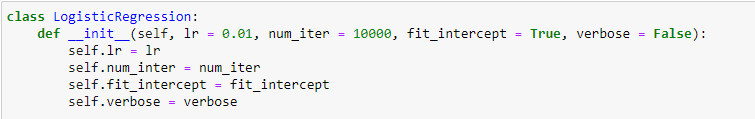
\includegraphics[width=\textwidth]{logistic_constructor.png}
    \caption{Konstruktor klase \texttt{LogisticRegression}}\label{fig:logconst}
\end{figure}

Funkcije koje enkapsulira klasa su sigmoidna funkcija (datu u jednačini \ref{eq:hypothesis}) koja daje predviđenu verovatnoću da instanca pripada pozitivnoj klasi i funkcija gubitaka koja smanjuje razliku između predviđene klase i klase kojoj trening instanca zaista pripada (datu u jednačini \ref{eq:loglossfinal}). Delovi koda koji prikazuju implementaciju dati su na slici \ref{fig:logsigloss}.

\begin{figure}[h]
    \centering
    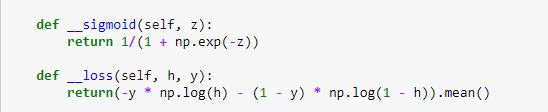
\includegraphics[width=0.8\textwidth]{logistic_sigmoid_loss.png}
    \caption{Implementacija sigmoidne funkcije i funkcije gubitaka klase \texttt{LogisticRegression}}\label{fig:logsigloss}
\end{figure}

Jedna od funkcija koja je izložena spoljnoj upotrebi je funkcija \texttt{fit}. Ova funkcija je kreirana po ugledu na funkcije iz biblioteke otvorenog koda \texttt{scikit-learn}. Ona služi za treniranje modela. Kao parametre ima matricu podataka obeleženu sa \textbf{X}, gde jedna vrsta matrice predstavlja jednu instancu, i vektor \textbf{y} koji sadrži labele za svaku instancu. Funkcija u okviru treniranja modela vrši predviđanja, nalazi gradijent funkcije u svakoj tački i onda optimizuje parametre $\theta$. To ponavlja određeni broj iteracija. Što je broj iteracija veći to 
će predviđanja biti preciznija, jer se će funkcija u svakoj iteraciji kretati bliže globalnom minimumu. Implementacija funkcije koja trenira model je data na slici \ref{fig:logfit}.

\begin{figure}[h]
    \centering
    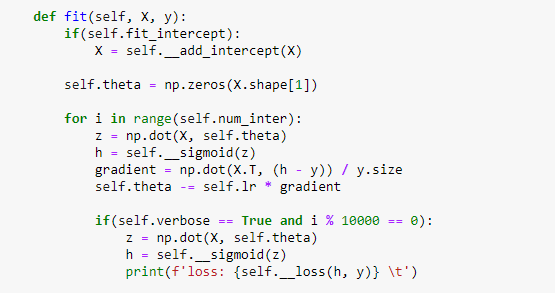
\includegraphics[width=0.8\textwidth]{logistic_fit.png}
    \caption{Implementacija funkcije za treniranje modela klase \texttt{LogisticRegression}}\label{fig:logfit}
\end{figure}

Nakon treniranja modela potrebno je da model može da vrši predviđanja za instance čije su labele nepoznate. Ovo se postiže funkcijama \texttt{predict prob} i \texttt{predict}. Obe klase imaju \texttt{public} modifikator pristupa što znači da bilo ko može da im pristupi. Funkcija \texttt{predict prob} uzima jednu instancu (vektor) ili više instanci (matricu)  i vraća predviđenu verovatnoću da instanca/instance pripada/ju pozitivnoj klasi. Funkcija \texttt{predict} takođe uzima kao parametar jednu instancu (vektor) ili više instanci (matricu) i vraća klasu koju je model predvideo da ta instanca/e pripada/ju.  Implementacija funkcija \texttt{predict prob} i \texttt{predict} je data na slici \ref{fig:logpred}.

\begin{figure}[h]
    \centering
    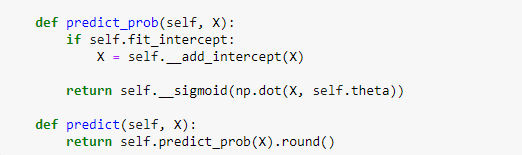
\includegraphics[width=0.8\textwidth]{logistic_predict.png}
    \caption{Implementacije funkcija \texttt{predict prob} i \texttt{predict} klase \texttt{LogisticRegression}}\label{fig:logpred}
\end{figure}

\subsection{Primena i analiza rezultata}
 \label{chap:primenalogistic}
 
U ovom delu ćemo implementirati projekat u kome ćemo klasu \texttt{LogisticRegression} za predikciju podataka. Glavni koraci pri izradi jednog projekta su: 
\begin{enumerate}
\item Pribavljanje podataka
\item Vizualizacija i upoznavanje podataka
\item Priprema podataka za obradu
\item Odabir modela i treniranje
\item Evaluacija modela
\item Testiranje modela
\end{enumerate}

\textbf{Pribavljanje i vizualizacija podataka}\\
 
Najčešći izvori podataka za analizu su relacione baze podataka. Vrlo često je potrebno da se podaci koji se nalaze u različitim tabelama denormalizuju i onda povežu u jednu logičku tabelu. U ovom projektu neće biti korišćeni podaci koji se nalaze u bazi podataka, već podaci u .csv formatu. Skup podataka koji će se koristiti je skup podataka o biljci perunici. Ovaj skup podataka od atributa sadrži dužinu i širinu čašičnog listića, kao i dužinu i širinu latice ove biljke. Uz ova četiri atributa takođe sadrži i informacije o vrsti perunike, odnosno labelu klase kojoj instanca pripada. Tri moguće klase, odnosno vrste perunike, kojima instance mogu da pripadaju su: \textit{Iris setosa, Iris virginica i Iris versicolor}. Skup podataka sadrži po 50 instanci svake klase. \\

Ovaj dataset je sastavni deo biblioteke scikit-learn i kod za njegovo učitavanje je dat na slici \ref{fig:irisload}.
\begin{figure}[h]
    \centering
    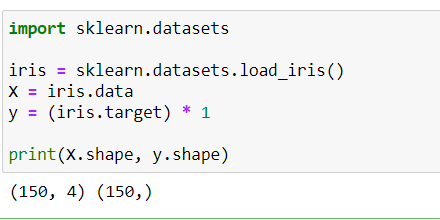
\includegraphics[width=0.8\textwidth]{iris_load.png}
    \caption{Učitavanje skupa podataka za perunike}\label{fig:irisload}
\end{figure}
 Na slici se vidi da je matrica \textbf{X} dimenzija 150x4, odnosno 150 instanci sa po četiri atributa. Vektor y sadrži 150 labela koje su oznake klase kojoj svaka instanca pripada.\\ 
 
Kako bi se stekao nekakav intuitivni osećaj za podatke, moguće je da se tabelarno prikaže prvih 5 elemenata skupa podataka. Ovo se u Pythonu postiže naredbom \texttt{head()}. Efekti naredbe su dati na slici \ref{fig:irishead}. Sa slike se može primetiti da su svi podaci mereni u cm.   
\begin{figure}[h]
    \centering
    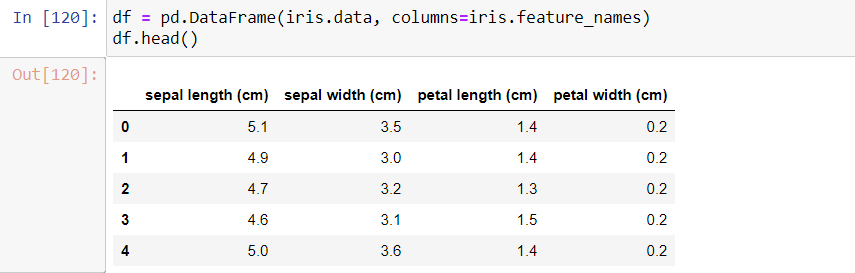
\includegraphics[width=0.8\textwidth]{iris_head.png}
    \caption{Prvih 5 elemenata skupa podataka}\label{fig:irishead}
\end{figure}

Naredbom \texttt{describe()} moguće je dobiti statističke podatke o skupu podataka. Funkcija vraća tabelu gde svaka kolona odgovara jednom atributu. U redovima tabele se nalaze informacije o broju instanci koje imaju ovaj podatak (gde je ova vrednost različita od null), o matematičkom očekivanju za taj atribut, o standardnoj devijaciji, o minimalnom i maksimalnom elementu skupa itd. Rezultat naredbe vidljiv je na slici \ref{fig:irisdescribe}.
\begin{figure}[h]
    \centering
    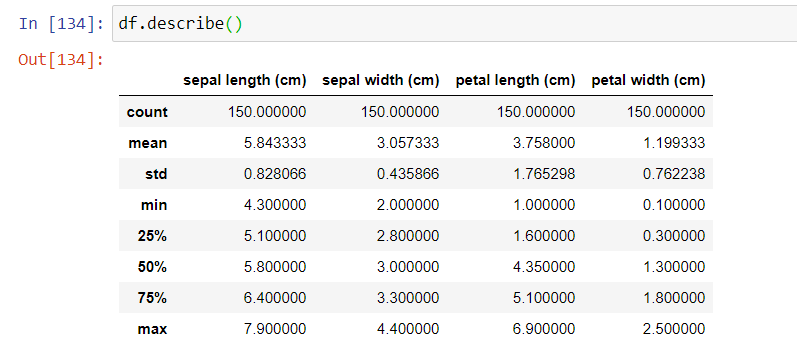
\includegraphics[width=0.8\textwidth]{iris_describe.png}
    \caption{Primena \texttt{describe} metode nad skupom podataka}\label{fig:irisdescribe}
\end{figure}

\begin{figure}[h]
    \centering
    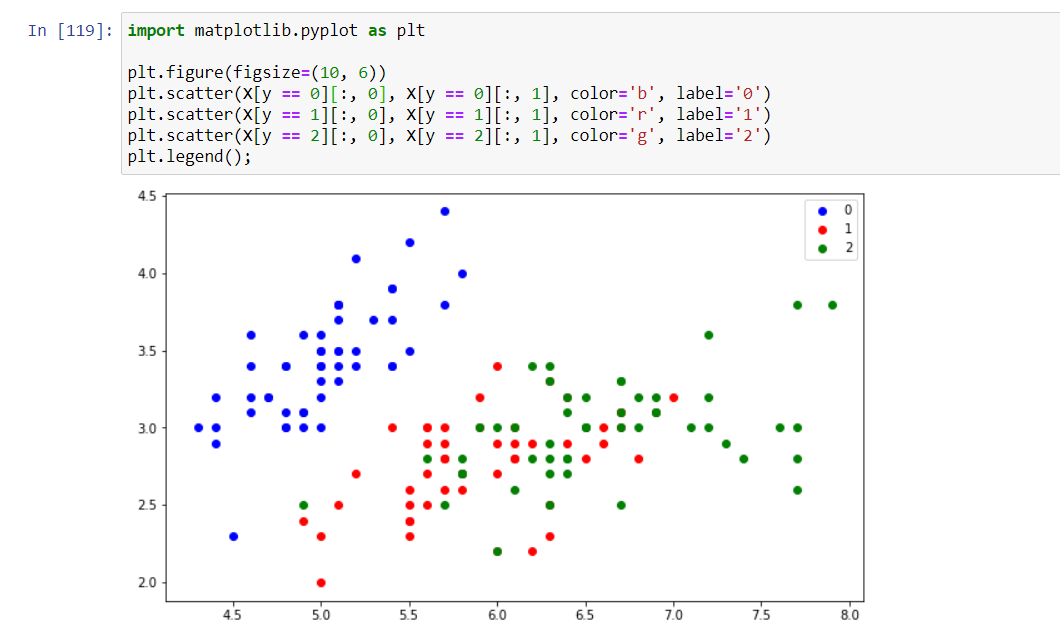
\includegraphics[width=0.8\textwidth]{iris_3_scatter.png}
    \caption{Vizuelizacija podataka za skup podataka o perunici}\label{fig:irisscatter}
\end{figure}

Vizualizacija podataka je jako važan korak pri upoznavanju skupa podataka. U Pythonu ovo se postiže funkcijama iz biblioteke otvorenog koda \textit{matplotlib}. Na grafiku na slici \ref{fig:irisscatter} na x osi imamo predstavljenu dužinu čašičnog listića, a na y osi širinu čašičnog listića. Instance su dobile boju na osnovu klase kojoj pripadaju. Vidimo da ako gledamo samo na osnovu ova dva atributa, klasa 1 čini jednu grupu, a klase 2 i 3 drugu grupu. Drugim rečima klase 1 i klase 2 i 3 su linearno razdvojive. Ovo je dobar problem za binarnu klasifikaciju i samim tim testiranje malopre implementirane klase za logističku regresiju. Model će biti treniran da prepoznaje da li instance pripadaju klasi 1 ili ne pripadaju. \\

\textbf{Priprema podataka i treniranje modela}\\

Pre nego što je neki skup podataka spreman da se njime trenira, i testira model, potrebno je podatke skalirati u neki opseg i rešiti se null vrednosti koje postoje u podacima. Skup podataka koji koristimo u ovom primeru je već prečišćen, odnosno skup podataka nema null vrednosti i sve su vrednosti otprilike istog reda veličine pa ih nema potrebe dalje skalirati. Treniranje modela je proces u kome se modelu, prosleđuje jedna po jedna ili čitava grupa instanci nekog skupa podataka sa labelama koje su oznake kojoj klasi pripadaju ili koju kontinualnu vrednost imaju kao labelu. Model ima funkciju kojom vrši predikciju labele za neku instancu. Zatim upoređuje labelu koju je predvideo sa labelom koja odgovara tom modelu. Ako se labele ne poklapaju model nekom metodom optimizacije optimizuje svoje parametre da bolje odgovaraju skupu podataka. Krajnji cilj je minimum funkcije koja se optimizuje tj da razlika između predviđene i stvarne vrednosti za labelu za sve instance bude minimalna. Pošto će isti skup podataka biti korišćen i za treniranje i za testiranje, potrebno ga je podeliti u test i trening skup podataka. Trening  i test skup podataka se deli u razmeri od 80:20. Trening skup podataka se koristi za treniranje modela, a test skup podataka za testiranje performansi modela. Funkcija koja će podeliti skup podatka u trening i test je data na slici \ref{fig:irissplit}.

\begin{figure}[h]
    \centering
    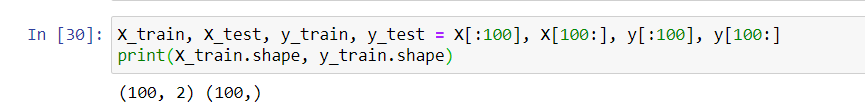
\includegraphics[width=0.8\textwidth]{iris_split_dataset.png}
    \caption{Podela podataka na trening i test skup}\label{fig:irissplit}
\end{figure}

Treniranje modela se vrši pozivanjem \texttt{fit()} funkcije instance klase \texttt{LogisticRegression}. Poziv funkcije za treniranje modela je dat na slici \ref{fig:logisticfitcall}. Funkciji se prosleduju vrednosti atributa u trening klasi i odgovarajuće labele. 

\begin{figure}[h]
    \centering
    
\includegraphics[width=0.8\textwidth]{logistic_fitcall.png}
    \caption{Podela podataka na trening i test skup}\label{fig:logisticfitcall}
\end{figure}

\textbf{Evaluacija modela}\\

Nakon treniranja modela potrebno je videti kakve performanse daje. Kod klasifikacionih modela glavne performanse mere su \textit{preciznost}, \textit{odziv}, \textit{matrica konfuzije}, \textit{f-mera} i \textit{ROC kriva}. U nastavku biće dat pregled svake od mera. \\

\textbf{Tačnost}\\

Tačnost je mera koja pokazuje koliko je ukupno istanci, od svih mogućih, klasifikator ispravno klasifikovao. To znači koliko je instanci pravilno raspodelio u pozitivnu i negativnu klasu u slučaju ovog binarnog klasifikatora. Da bi se izbegla pristrasnost klasifikatora pri evaluaciji modela najčešće se  koristi \textit{k-fold cross validation} metoda. Trening skup podataka, najčešće se on korisiti za validaciju, ova metoda deli na \textit{k} skupova. Pri evaluaciji modela ovom metodom, treniranje modela se radi k puta. U svakoj iteraciji jedan od k skupova, (svaki put različiti, tako da na kraju treniranja svi dođu na red) se uzima da bude validacioni skup. Ostalih k-1 su trening skupovi. Kada se model istrenira, na validacionom skupu se proverava tačnost klasifikatora. Implementacija i primena k-fold cross validation funkcije je data na slici \ref{fig:logisticprecission}.

\begin{figure}[h]
    \centering
    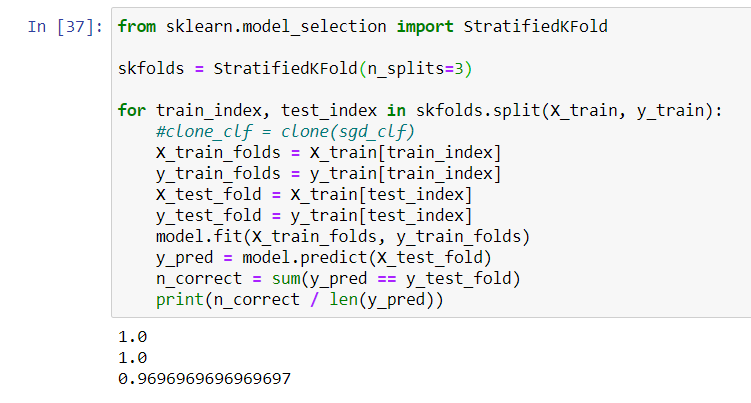
\includegraphics[width=0.8\textwidth]{logistic_precision.png}
    \caption{K fold cross validation funkcija u evaluaciji modela}\label{fig:logisticprecission}
\end{figure}

U ovom slučaju se trening skup deli na tri dela i rezultati tačnosti su redom 1.0, 1.0 i 0.97, što je jako dobar rezultat.\\

\textbf{Matrica konfuzije}\\

Mnogo temeljniji način za evaluaciju performansi klasifikatora je matrica konfuzije. Matrica konfuzije nam govori koliko je instanci jedne klase klasifikovano kao instanca neke druge klase. Na glavnoj dijagonali se nalazi broj ispravno klasifikovanih instanci, odnosno za binarni klasifikator TP (True Positive - instance koje su klasifikovane kao pozitivne i čija je labela pozitivna, ispravno klasifikovane pozitivne instance) i TN (True Negative - 
instance koje su klasifikovane kao negativne i čija je labela negativna). Na slici \ref{fig:confussion} je dat šematski prikaz matrice konfuzije za binarni klasifikator. Polje FN (False Negatives) prikazuje broj elemenata čija je predviđena klasa negaitvna, a koji zapravo pripadaju pozitivnoj klasi.  Polje FP (False Positives) prikazuje broj elemenata čija je predviđena klasa pozitivna, a koji zapravo pripadaju negativnoj klasi.\\

\begin{figure}[h]
    \centering
    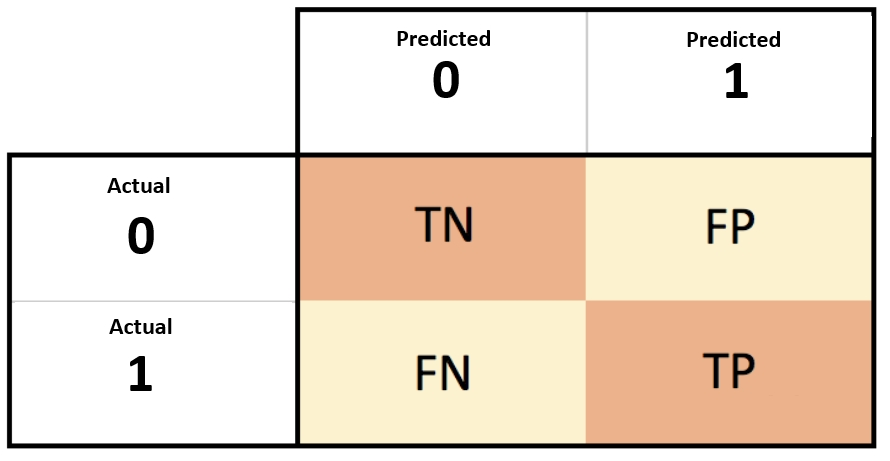
\includegraphics[width=0.6\textwidth]{confusion_matrix.jpg}
    \caption{Primer matrice konfuzije}\label{fig:confussion}
\end{figure}

Matrica konfuzije za model logističke regresije primenjen na skup podataka za peruniku je dat na slici \ref{fig:confusioniris}.

\begin{figure}[h]
    \centering
    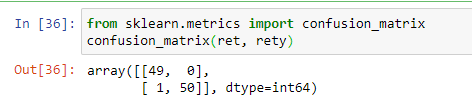
\includegraphics[width=0.6\textwidth]{logistic_confusion.png}
    \caption{Matrica konfuzije za model logističke regresije nad skupom podataka vezanim za perunike}\label{fig:confusioniris}
\end{figure}

Zaključak koji se može izvesti iz matrice konfuzije \ref{fig:confusioniris} je da po 1/3 instanci pozitivne i negativne klase klasifikator ne prepoznaje, što nije tako idealan rezultat.\\

\textbf{Preciznost, odziv i f-mera}\\

Jedna od metrika koja se može dobiti iz matrice konfuzije je preciznost. Preciznost klasifikatora je tačnost pozitivnih predviđanja. Jednačinom \ref{eq:accuracy} se računa preciznost klasifikatora. 

\begin{equation} \label{eq:accuracy}
	preciznost = \frac{TP}{TP + FP} = \frac{50}{1 + 50} = 0.98
\end{equation}

Preciznost je 0.67, odnosno od ukupnog broja instanci za koje je klasifikator rekao da su pozitivne, samo 67\% je stvarno pozitivno. 

\begin{equation} \label{eq:recall}
	odziv = \frac{TP}{TP + FN} = \frac{50}{0 + 50} = 1
\end{equation}-

Jednačinom \ref{eq:recall} se računa odziv. Odziv predstavlja odnos između instanci koje je klasifikator prepoznao kao pozitivne i koje stvarno jesu pozitivne i ukupnog broja stvarno pozitivnih instanci u skupu podataka. Ovaj model ima preciznost 0.68\%, što znači da je od svih mogućih pozitivnih instanci model prepoznao samo 68\%.

\begin{equation} \label{eq:f-measure}
	f-mera = \frac{2}{\frac{1}{preciznost} + \frac{1}{odziv}} =  \frac{2}{\frac{1}{0.98} + \frac{1}{1}} = 0.99
\end{equation}

F mera je potrebna kada je poželjno kombinovati odziv i preciznost u jednu meru. F mera je harmonijska sredina preciznosti i odziva (jednačina \ref{eq:f-measure}). Obično se koristi kada je potreban brz i jednostavan način da se uporede dva klasifikatora. Iz jednačine se vidi da će F mera imati visoku vrednost samo ako su i preciznost i odziv visoki. \\

\textbf{ROC kriva}\\

ROC kriva (engl. \textit{Receiver operating characteristic} je još jedan važan alat pri evaluaciji binarnih klasfikatora. Na x-osi se nalazi True Positive Rate (odziv), a na y osi False Positive Rate (odnos negativnih instanci koje su pogrešno klasifikovane kao pozitivne). Idealni klasifikator ima površinu ispod ROC krive jednaku 1. ROC kriva za ovaj klasifikator je data na slici \ref{fig:logisticroc}. Površina ispod krive je data na slici \ref{fig:logisticrocscore}.\\

\begin{figure}[h]
    \centering
    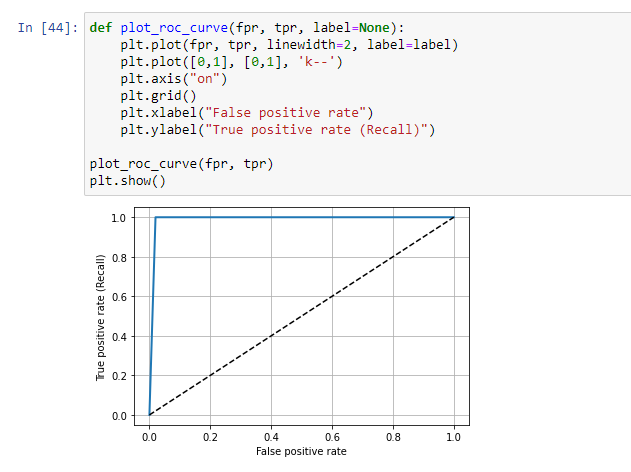
\includegraphics[width=0.8\textwidth]{logistic_roc.png}
    \caption{ROC kriva}\label{fig:logisticroc}
\end{figure}

\begin{figure}[h]
    \centering
    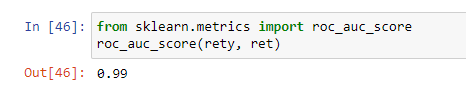
\includegraphics[width=0.8\textwidth]{logistic_roc_score.png}
    \caption{Površina ispod ROC krive}\label{fig:logisticrocscore}
\end{figure}

\textbf{Testiranje modela}\\

Testiranje modela se radi tako što se podaci iz dela skupa podataka koji su odvojeni testiranje daju modelu. Model generiše predikcije za te podatke. Zatim računa preciznost klasifikatora na test skupu podataka. Primena testiranja i preciznost klasifikatora su dati na slici \ref{fig:logistictesting}. 

\begin{figure}[h]
    \centering
    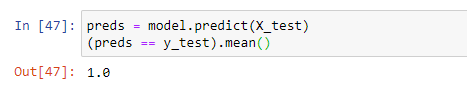
\includegraphics[width=0.6\textwidth]{logistic_testing.png}
    \caption{Testiranje modela logističke regresije i preciznost}\label{fig:logistictesting}
\end{figure}

Preciznost klasifikatora nad test podacima je 1, što znači da su sve instance test skupa ispravno klasifikovane. \\

\section{Softmaks regresija}

U nastavku biće data kompletna implementacija softmaks regresije u programskom jeziku Python. Regresija je implementirana kao klasa \texttt{Softmax Regression}. Metode koje instanca ove klase može javno pozivati su metoda \texttt{fit} i \texttt{predict}. Metoda \texttt{fit} omogućava treniranje modela softmaks regresije. Metoda \texttt{predict} omogućava da se vrši predikcija za podatke čija je klasa nepoznata. Skup podataka koji je korišćen za testiranje modela je takođe \textit{iris} skup podataka. U ovom slučaju smo umesto dve klase koristili sve tri, tako da i za predikciju imamo sve tri vrste klasa.

\subsection{Opis klase}

Funkcionalnosti softmaks regresije su enkapsulirane u klasi \texttt{SoftmaxRegression}. Klasa izlaže konstruktor u kome se prosleđuje broj interacija i parametar $\alpha$ koji predstavlja brzinu učenja (engl. \textit{learning rate}). Uz ova dva parametra prosleđuje se i broj klasa koji postoji u skupu podataka, kao parametar \textit{K}. Na slici \ref{fig:softmaxconst} je dat prikaz konstruktora klase \texttt{SoftmaxRegression}.

\begin{figure}[h]
    \centering
    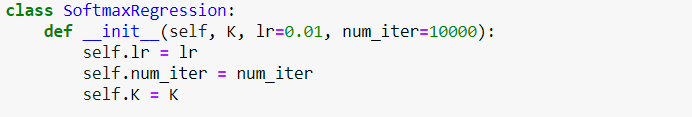
\includegraphics[width=\textwidth]{softmax_constructor.png}
    \caption{Konstruktor klase \texttt{SoftmaxRegression}}\label{fig:softmaxconst}
\end{figure}

Funkcije koje enkapsulira klasa su softmaks funkcija (datu u jednačini \ref{eq:softmax}) koja daje predviđenu verovatnoću da instanca pripada pozitivnoj klasi i funkcija gubitaka koja smanjuje razliku između predviđene klase i klase kojoj trening instanca zaista pripada (datu u jednačini \ref{eq:crossentropy}). Delovi koda koji prikazuju implementaciju dati su na slici \ref{fig:softmaxpred}.

\begin{figure}[h]
    \centering
    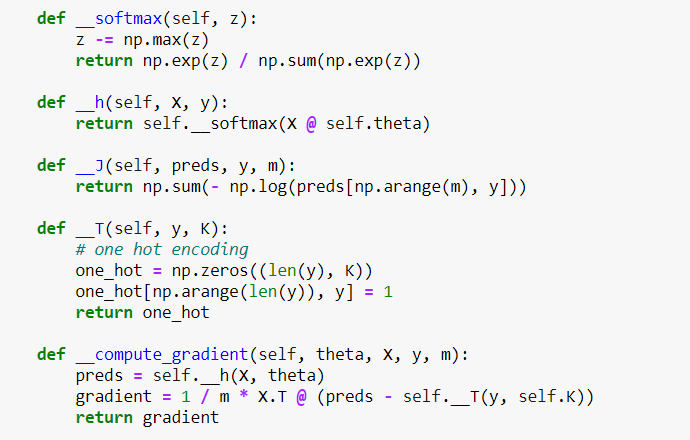
\includegraphics[width=0.6\textwidth]{softmax_predict.png}
    \caption{Implementacija softmaks funkcije i funkcije gubitaka klase \texttt{SoftmaxRegression}}\label{fig:softmaxpred}
\end{figure}

Jedna od funkcija koja je izložena spoljnoj upotrebi je funkcija \texttt{fit}. Ona služi za treniranje modela. Kao parametre ima matricu podataka obeleženu sa \textbf{X}, gde jedna vrsta matrice predstavlja jednu instancu, i vektor \textbf{y} koji sadrži labele za svaku instancu. Funkcija u okviru treniranja modela vrši predviđanja, nalazi gradijent funkcije u svakoj tački i onda optimizuje parametre $\theta$. To ponavlja određeni broj iteracija. Što je broj iteracija veći to će predviđanja biti preciznija, jer se će funkcija u svakoj iteraciji kretati bliže globalnom minimumu. Implementacija funkcije koja trenira model je data na slici \ref{fig:softfit}.

\begin{figure}[h]
    \centering
    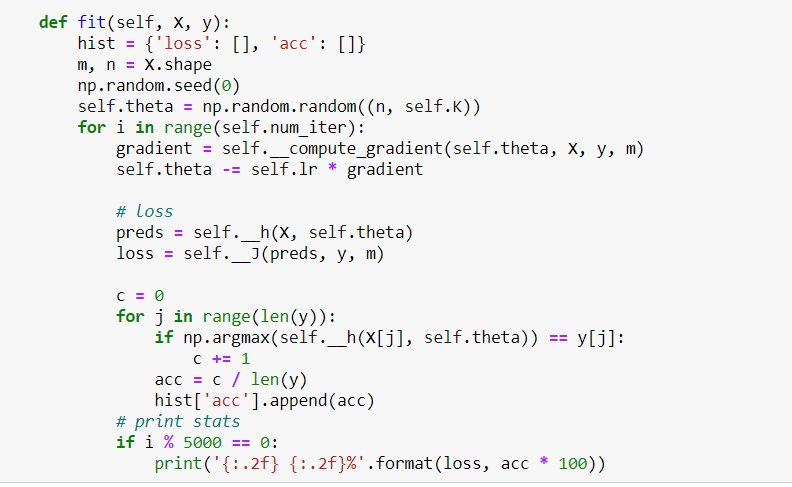
\includegraphics[width=0.8\textwidth]{softfit.png}
    \caption{Implementacija funkcije za treniranje modela klase \texttt{SoftmaxRegression}}\label{fig:softfit}
\end{figure}

Nakon treniranja modela potrebno je da model može da vrši predviđanja za instance čije su labele nepoznate. Ovo se postiže funkcijama \texttt{predict prob} i \texttt{predict}. Obe klase imaju \texttt{public} modifikator pristupa što znači da bilo ko može da im pristupi. Funkcija \texttt{predict prob} uzima jednu instancu (vektor) ili više instanci (matricu)  i vraća predviđenu verovatnoću da instanca/instance pripada/ju pozitivnoj klasi. Funkcija \texttt{predict} takođe uzima kao parametar jednu instancu (vektor) ili više instanci (matricu) i vraća klasu koju je model predvideo da ta instanca/e pripada/ju.  Implementacija funkcija \texttt{predict prob} i \texttt{predict} je data na slici \ref{fig:softpred}.

\begin{figure}[h]
    \centering
    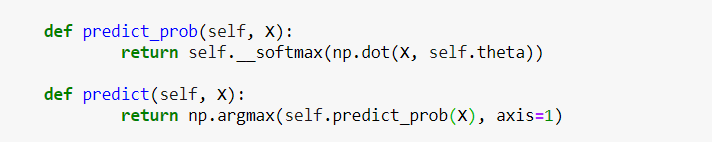
\includegraphics[width=0.8\textwidth]{softpred.png}
    \caption{Implementacije funkcija \texttt{predict prob} i \texttt{predict} klase \texttt{SoftmaxRegression}}\label{fig:softpred}
\end{figure}

\subsection{Primena i analiza rezultata}

Softmaks regresija je vrsta višeklasne regresije. Kod višeklasne regresije postoji više klasa za koje se instance klasifikuju. Jedna instanca uvek pripada jednoj klasi. \\ 

U ovom delu ćemo implementirati projekat u kome ćemo klasu \texttt{SoftmaxRegression} za predikciju podataka. Za treniranje i implementaciju modela koristićemo isti skup podataka o perunikama kao za logističku regresiju. U narednoj sekciji ćemo se kratko osvrnuti na proces treniranja modela, evaluaciju i testiranje modela. Pošto je skup podataka isti deo koji se odnosi na pribavljanje podataka, vizuelizaciju i pripremu podataka biće izostavljen, pošto je već priložen u sekciji \ref{chap:primenalogistic}. \\

\textbf{Treniranje i evaluacija modela}\\

Za treniranje modela podelićemo skup podataka u dva podskupa. Podskup za treniranje će sadržati 140 instanci, a podskup za testiranje će sadržati samo 10 instanci. Podela skupa podataka na trening i test skup data je na slici \ref{fig:softsplit}. \\

\begin{figure}[h]
    \centering
    
\includegraphics[width=0.7\textwidth]{softmax_split_train_test.png}
    \caption{Podela skupa podataka na trening i test skup za softmaks regresiju}\label{fig:softsplit}
\end{figure}

Treniranje modela se radi funkcijom \texttt{fit()}. Poziv funkcije za treniranje modela je dat na slici \ref{fig:softtrain}. \\

\begin{figure}[h]
    \centering
    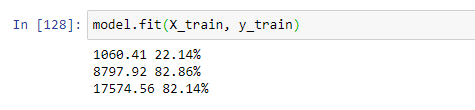
\includegraphics[width=0.7\textwidth]{softmax_train.png}
    \caption{Podela skupa podataka na trening i test skup za softmaks regresiju}\label{fig:softtrain}
\end{figure}

Nakon treniranja modela, za evaluaciju biće prikazane metrike poput matrice konfuzije, preciznosti, odziva i f-mere. Vrednosti za sve ove mere biće generisane preko biblioteke scikit-learn. Kod kojim se dobijaju je dat na slici \ref{fig:softmaxeval}. \\

\begin{figure}[h]
    \centering
    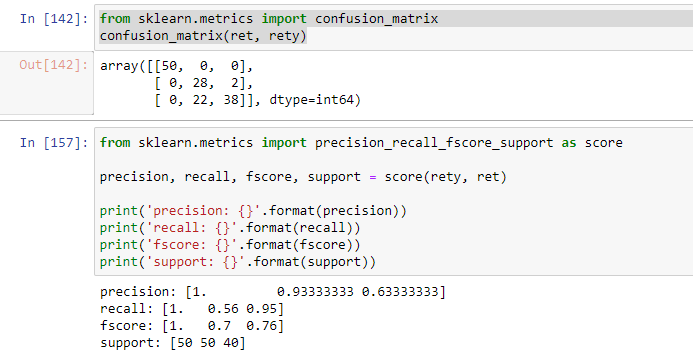
\includegraphics[width=0.7\textwidth]{softmax_evaluation.png}
    \caption{Evaluacija modela za softmaks regresiju}\label{fig:softmaxeval}
\end{figure}

Iz matrice konfuzije se jasno vidi da model savršeno prepoznaje instance prve klase, međutim meša instance koje pripadaju klasi 2 i 3. Ovo je bila činjenica koju smo eksploatisali kada smo ovaj skup podataka koristili da logističkom regresijom radimo binarnu klasifikaciju za klasu 1. Da bi se izbegla pristrasnost klasifikatora pri evaluaciji modela najčešće se koristi \textit{k-fold cross validation} metoda. Korišćenjem metode \texttt{precision recall fscore support()} iz biblioteke sklearn, dobićemo preciznost, odziv f meru za svaku od klasa. Iz priloženih metrika se jasno vidi da model savršeno prepoznaje sve instance klase 1, a da meša instance klase 2 i 3. Preciznost je najlošija za klasu 3, što znači da od svih instanci koje je klasifikator prepoznao kao da pripadaju klasi 3, samo 63\% zaista pripada klasi 3. Najlošiji odziv ima klasa 2, što znači da je klasifikator od svih instanci koje pripadaju klasi 2, samo njih 56\% prepoznao kao da pripadaju klasi 2. \\

\textbf{Testiranje modela}\\

Testiranje modela se radi sa 10 instanci koje su izdvojene iz početnog skupa podataka. Kod kojim se instance prosleđuju istreniranom modelu je dat na slici \ref{fig:softmaxtest}

\begin{figure}[h]
    \centering
    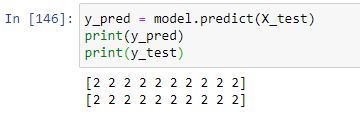
\includegraphics[width=0.7\textwidth]{softmax_test.png}
    \caption{Testiranje modela za softmaks regresiju}\label{fig:softmaxtest}
\end{figure}

Modelu su prosleđene instance koje pripadaju klasi 2, i on ih je sve ispravno klasifikovao. \\

\chapter{Primena kod neuronskih mreža}

\end{document}